\section{Aluminiumoxid-ALD}
\label{aluminaald}

Einen beispielhaften Prozess für Atomlagenabscheidungen bildet die Abscheidung von Aluminiumoxid \ce{Al2O3}\cite{puurunen_surface_2005}, für die häufig das Precursorpaar Trimethylaluminium (TMA, \ce{Al(CH4)3}) und Wasser genutzt wird.
Mit einer Permittivität von $k=\approx 8$ hat Aluminiumoxid neben anderen Materialien das zuvor geläufige Siliziumdioxid ($k=3.9$) in der Halbleiterindustrie etwa in modernen Prozessoren ersetzt, obwohl die Reaktionsmechanismen nicht vollends verstanden sind\todo{dringend ref!}.
Deshalb soll der TMA-\ce{H2O}-Prozess im Folgenden untersucht werden, allerdings ist seine vollständige Simulation per Parsivald mit vollständigen Precursormolekülen bisher nicht gelungen.

\subsection{Precursor-Simulationen}

Die Zahl der verfügbaren Parametrisierungen reduziert sich für \ce{Al2O3} auf drei Kandidaten, die bereits aus den Untersuchungen der Silizium-Potentiale bekannt sind:\\
\todo{Stil ok?}\texttt{Al\_AlO\_AlN}, \texttt{liu\_ettringite}, das nachfolgend nur unter der Bezeichnung \texttt{liu} geführt werden soll, und \texttt{narayanan}.

Die Al\_AlO\_AlN-Datei stammt direkt aus der offiziellen LAMMPS-Distribution, wurde jedoch spätestens in der Version vom 17. Dezember 2014 aus dem Paket genommen, was vermutlich durch die schlechte Darstellung der Materialeigenschaften von Bulk-Materialien liegt, wie nachfolgend untersucht wird.

Bei der Liu-Potentialdatei rührt die Unterstützung für sowohl Aluminium als auch Silizium von der Abwandlung einer bestehender Parametrisierungen, die bereits Silizium unterstützt hat.
Da jedoch bei der Erweiterung auf Ettringit (\ce{Ca6[Al(OH)6]2(SO4)3 26H2O}) die Konsistenz der Silizium-Parameter nicht bewahrt wurde, können Silizium-Materialien damit nicht verlässlich simuliert werden, wie in Abschnitt \ref{siliconpvd} gezeigt wurde.
Ettringit hingegen enthält \ce{Al}-\ce{O}-Bindungen und \ce{OH}-Gruppen, so dass zumindest die Simulation des Bulkmateriales und einer hydroxylierten Oberfläche aussichtsreich erscheint.

Die Narayanan-Parametrisierung lässt aufgrund ihrer Herkunft als Potential für \ce{Li-Al}-Silikate für die Simulation von Eukryptit (\ce{LiAl[SiO4]}) endgültige Aussage über die Qualität der \ce{Al}-\ce{O}-Bindungen und \ce{OH}-Gruppen zu.
Zwar besteht der Trainingssatz aus Lithium-Aluminium-Kristallen, aber nur $\gamma$-\ce{LiAlO2} beinhaltet direkte \ce{Al}-\ce{O}-Bindungen, während keine der für das Fitting genutzten Strukturen Wasserstoff beinhaltet hat.
Es ist daher unwahrscheinlich, dass die Narayanan-Potentialdatei komplizierte Systeme verlässlich darstellt.

\subsection{Precursor-Oberflächen-Reaktionen}

Der erste Schritt in der Simulation von Aluminiumoxid ist \todo{continuehere}

\begin{figure}
  \captionsetup[subfigure]{singlelinecheck=false}
  \def\subfigwidth{0.32\textwidth}
  \begin{subfigure}[t]{\subfigwidth}
    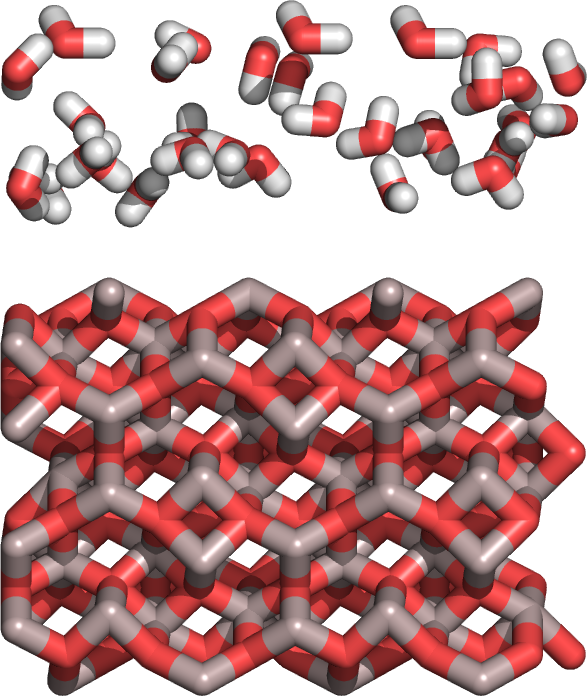
\includegraphics[width=\textwidth]{alumina_h2o_before}
    \subcaption{Seitenansicht, vorher}
  \end{subfigure}
  \hfill
  \begin{subfigure}[t]{\subfigwidth}
    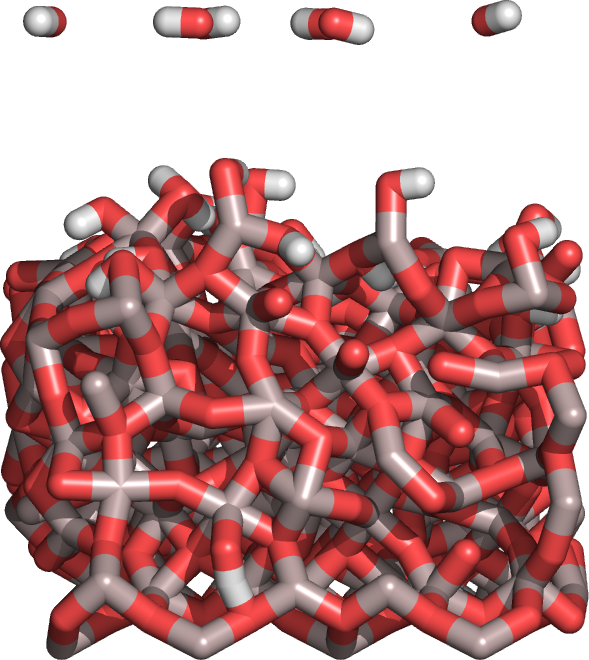
\includegraphics[width=\textwidth]{alumina_h2o_after}
    \subcaption{Seitenansicht, nachher}
  \end{subfigure}
  \hfill
  \begin{subfigure}[t]{\subfigwidth}
    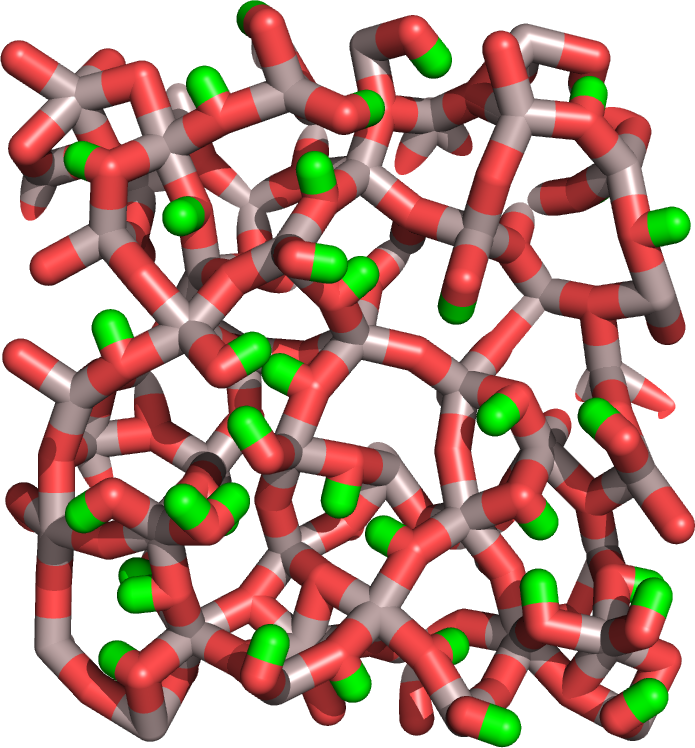
\includegraphics[width=\textwidth]{alumina_h2o_topview}
    \subcaption{Draufsicht, nachher.
      Hydroxyl ist grün hervorgehoben.
    }
  \end{subfigure}
  \caption[Oberflächenreaktion von Wasser mit $\alpha$-\ce{Al2O3}]{Ergebnisse einer Oberflächenreaktion von Wasser mit $\alpha$-\ce{Al2O3}.
    Das Wasser reagiert mit Sauerstoffatomen an der Oberfläche zu Hydroxylgruppen.
  }
  \label{fig:wateraluminasurface}
\end{figure}

\subsection{Vollständige ALD-Simulationen}

\todo[inline]{Erklären, warum es vermutlich noch nicht geht}
